\documentclass{article}
\usepackage[margin=1in]{geometry}
\usepackage{amsmath, amssymb, amsthm}
\usepackage{enumitem}

% colored links
\usepackage{hyperref}
\hypersetup{
    colorlinks=true,
    linkcolor=blue,
    filecolor=magenta,      
    urlcolor=magenta,
    }


% Inputting Python code
\usepackage[dvipsnames]{xcolor}
\definecolor{textblue}{rgb}{.2,.2,.7}
\definecolor{textred}{rgb}{0.54,0,0}
\definecolor{textgreen}{rgb}{0,0.43,0}
\usepackage{upquote}
\usepackage{listings}
\lstset{
    language=Python, 
    tabsize=4,
    basicstyle={\ttfamily},
    keywordstyle=\color{textblue},
    commentstyle=\color{textgreen},
    stringstyle=\color{textred},
    frame=none,
    columns=fullflexible,
    keepspaces=true,
    showstringspaces=false,
    xleftmargin=-15mm, % manual adjustment, figure out permanent solution
}

\newcommand{\gray}[1]{\textcolor{gray}{#1}}

%Creating algorithms
\usepackage{algorithm}
\usepackage[noend]{algpseudocode}

\usepackage{tcolorbox}
\tcbuselibrary{skins,hooks}
\usetikzlibrary{shadows}
\usepackage{lipsum}

%Images
\usepackage{graphicx}
    \usepackage{subcaption}
    \usepackage{float}
    % \usepackage[labelsep=period]{caption}

    
%Creating Figures
\usepackage{tikz}
\usetikzlibrary{calc, math, matrix, graphs, positioning}


% the settings of tikz is used for the optimization of the graphs  
\usetikzlibrary{shapes, arrows, calc, arrows.meta, fit, positioning} % these are the parameters passed to the library to create the node graphs  
\tikzset{  
    auto,node distance =1.1 cm and 1.1 cm,% node distance is the distance between one node to other, where 1.5cm is the length of the edge between the nodes  
    state/.style ={ellipse, draw, minimum width = 0.9 cm}, % the minimum width is the width of the ellipse, which is the size of the shape of vertex in the node graph  
    point/.style = {circle, draw, inner sep=0.18cm, fill, node contents={}},  
    el/.style = {inner sep=2.5pt, align=right, sloped}  
}  

%Formatting and Spacing
\setitemize[1]{noitemsep, parsep = 5pt, topsep = 5pt}
\setenumerate[1]{label = (\alph*), parsep = 1pt, topsep = 5pt}
\setlength\parindent{0pt}
\linespread{1.1}

% title
\title{\vspace{-1cm}CS 2051: Honors Discrete Mathematics \\Spring 2023 Homework 5 Supplement Solution}
\author{Sarthak Mohanty }
\date{}

\begin{document}

\maketitle

The \lstinline{generate_schedule} method in this supplement seemed to pose quite the challenge! In this short document, we cover some initial approaches, the challenges/issues encountered, the correct approach, and an explanation on why it works

\begin{center}
    \textbf{Incorrect Approach}
\end{center}

A common approach was modifying Kahn's algorithm as follows:
\begin{itemize}
    \item initialize final schedule $L = []$
    \item loop until all tasks scheduled:
    \begin{itemize}
        \item Find all current minimal elements in poset, remove them from \lstinline{poset} and put them in one list $\ell$
        \item If $|\ell| >$ \lstinline{num_processors}, split $\ell$ into multiple lists $\ell_{1}, \dots, \ell_{i}$.
        \item add these lists to $L$
    \end{itemize}
\end{itemize}

This approach works fine for the example given in the docstrings, as shown below:
    \begin{center}
        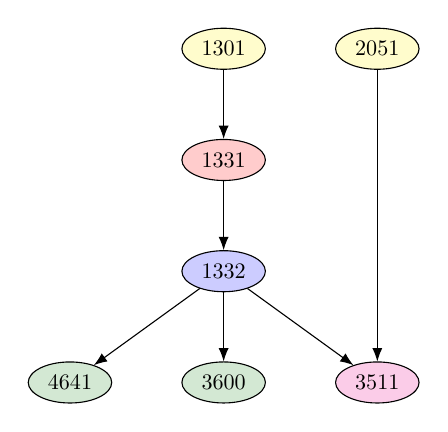
\begin{tikzpicture}[scale = 0.8, transform shape]  
            \node[state, fill=yellow!20] (1301) at (0,0) {1301}; % here, state signifies that the shape of the node will be the shape declared in the above state/.style command.  
            \node[state,fill=red!20] (1331) [below =of 1301] {1331};  
            \node[state, fill=blue!20] (1332) [below =of 1331] {1332};
            \node[state, fill=yellow!20] (2051) [right =of 1301] {2051};  
            \node[state, fill=ForestGreen!20] (3600) [below =of 1332] {3600};  
            \node[state, fill=ForestGreen!20] (4641) [left =of 3600] {4641};
            \node[state, fill=magenta!20] (3511) [right =of 3600] {3511};  
            \path[-Latex] (1301) edge (1331); % it is the path of the edge from one node to another  
            \path[-Latex] (1331) edge (1332);
            \path[-Latex] (1332) edge (4641);
            \path[-Latex] (1332) edge (3600);
            \path[-Latex] (1332) edge (3511);
            \path[-Latex] (2051) edge (3511);
        \end{tikzpicture}
    \end{center}


\begin{tcolorbox}[enhanced,title=My title,
colframe=red!50!black,colback=red!10!white,
arc=1mm,colbacktitle=red!10!white,
fonttitle=\bfseries,coltitle=red!50!black,
attach boxed title to top left ={yshift=-0.50mm},
boxed title style={skin=enhancedfirst jigsaw,
size=small,arc=1mm,bottom=-1mm,
interior style={fill=none,
top color=red!30!white,
bottom color=red!20!white}}]
    This is a \textbf{tcolorbox}.
\end{tcolorbox}

\begin{tcolorbox}[enhanced,title=My title,
attach boxed title to bottom text left]
This is a \textbf{tcolorbox}.
\end{tcolorbox}

    \begin{lstlisting}[belowskip=-10pt]
        >>> generate_schedule({'1301', '1331', '1332', '4641', '2051', '3600', '3511'},
                {('1301', '1331'), ('1331', '1332'), ('1332', '4641'),\
                 ('2051', '3511'), ('1332', '3511'), ('1332', '3600')}, 2)
            ['1301', '2051'], ['1331'], ['1332'], ['4641', '3600'], ['3511']]]
    \end{lstlisting}

\begin{center}
    \textbf{The Issue}
\end{center}

    \begin{center}
        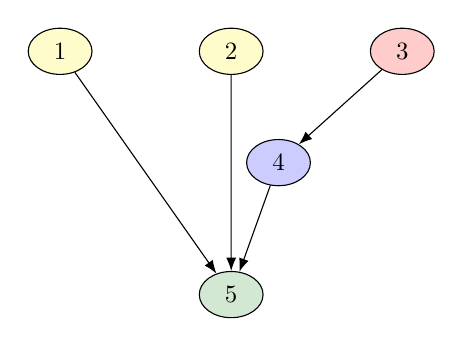
\begin{tikzpicture}[scale = 0.9, transform shape]  
            \node[state, fill=yellow!20] (1) at (0,0) {1};
            \node[state,fill=yellow!20] (2) [right = of 1, right=1.5cm] {2};  
            \node[state, fill=red!20] (3) [right = of 2, right=1.5cm] {3};
            \node[state, fill=blue!20] (4) [below left =of 3,] {4};  
            \node[state, fill=ForestGreen!20] (5) [below of =2, below=2cm] {5}; 
            \path[-Latex] (1) edge (5);
            \path[-Latex] (2) edge (5);
            \path[-Latex] (3) edge (4);
            \path[-Latex] (4) edge (5);
        \end{tikzpicture}
    \end{center}
% https://tikz.dev/tikz-trees
    \begin{center}
        \begin{tikzpicture}[scale = 0.9, transform shape]  
         
            \node[state, fill=ForestGreen!20] (5) [above of =2, above=2cm] {5}; 
            \node[state, fill=blue!20] (4) [right=of 2] {4};
            \node[state, fill=red!20] (3) [below right=of 3] {3};
            \node[state,fill=yellow!20] (2) [right = of 1, right=1.5cm] {2};
            \node[state, fill=yellow!20] (1) at (0,0) {1};   
            \path[-Latex] (1) edge (5);
            \path[-Latex] (2) edge (5);
            \path[-Latex] (3) edge (4);
            \path[-Latex] (4) edge (5);
        \end{tikzpicture}
    \end{center}

\begin{center}
    \textbf{Correct Approach}
\end{center}


\begin{figure}[htbp]
    \centering
    
    \begin{subfigure}{.45\textwidth}
        \centering
        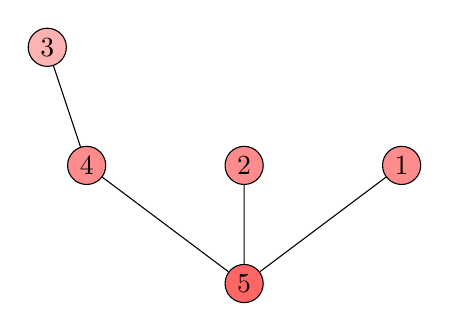
\begin{tikzpicture}
            [level distance=15mm,
            every node/.style={fill=red!60,circle,inner sep=2pt},
            level 1/.style={sibling distance=20mm,nodes={fill=red!45}},
            level 2/.style={sibling distance=10mm,nodes={fill=red!30}},
            level 3/.style={sibling distance=5mm,nodes={fill=red!25}}]
            % \node [missing]
            %     child {node [draw] {1} }
                
            %     child {node [draw] {2} }
            %     child {node [draw] {3}
            %         child {node [draw] {4} }
            %         child [missing]
            %     };
            \node [draw] {5} [grow=up]
                child {node [draw] {1} }
                child {node [draw] {2} }
                child {node [draw] {4}
                    child[missing]
                    child {node [draw] {3} }
                };
        \end{tikzpicture}
    \end{subfigure}
    \begin{subfigure}{.45\textwidth}
        \centering
        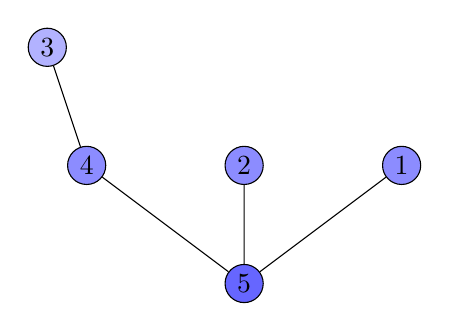
\begin{tikzpicture}
            [level distance=15mm,
            every node/.style={fill=blue!60,circle,inner sep=2pt},
            level 1/.style={sibling distance=20mm,nodes={fill=blue!45}},
            level 2/.style={sibling distance=10mm,nodes={fill=blue!30}},
            level 3/.style={sibling distance=5mm,nodes={fill=blue!25}}]
            \node [draw] {5} [grow=up]
                child {node [draw] {1} }
                child {node [draw] {2} }
                child {node [draw] {4}
                    child[missing]
                    child {node [draw] {3} }
                };
        \end{tikzpicture}
    \end{subfigure}
    \caption{Two examples of binary trees. The tree on the left is full, while the tree on the right is not.}
    \label{fig:Q3}
\end{figure}


\begin{figure}[htbp]
        \centering
        
        \begin{subfigure}{.45\textwidth}
            \centering
            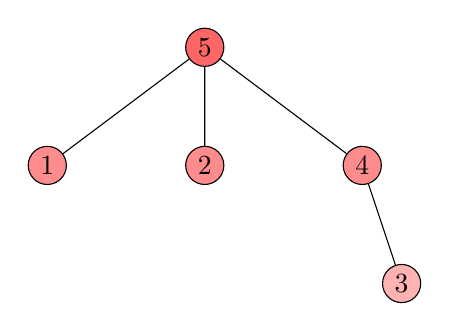
\begin{tikzpicture}
                [level distance=15mm,
                every node/.style={fill=red!60,circle,inner sep=2pt},
                level 1/.style={sibling distance=20mm,nodes={fill=red!45}},
                level 2/.style={sibling distance=10mm,nodes={fill=red!30}},
                level 3/.style={sibling distance=5mm,nodes={fill=red!25}}]
                \node [draw] {5}
                    child {node [draw] {1} }
                    child {node [draw] {2} }
                    child {node [draw] {4}
                        child[missing]
                        child {node [draw] {3} }
                    };
            \end{tikzpicture}
        \end{subfigure}
        \begin{subfigure}{.45\textwidth}
            \centering
            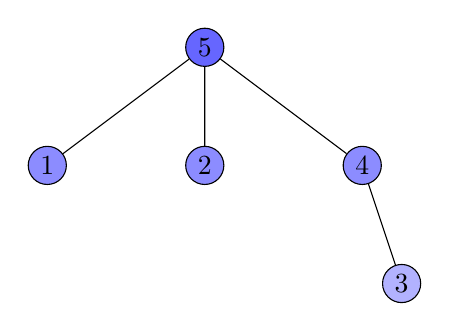
\begin{tikzpicture}
                [level distance=15mm,
                every node/.style={fill=blue!60,circle,inner sep=2pt},
                level 1/.style={sibling distance=20mm,nodes={fill=blue!45}},
                level 2/.style={sibling distance=10mm,nodes={fill=blue!30}},
                level 3/.style={sibling distance=5mm,nodes={fill=blue!25}}]
                \node [draw] {5}
                    child {node [draw] {1} }
                    child {node [draw] {2} }
                    child {node [draw] {4}
                        child[missing]
                        child {node [draw] {3} }
                    };
            \end{tikzpicture}
        \end{subfigure}
        \caption{Two examples of binary trees. The tree on the left is full, while the tree on the right is not.}
        \label{fig:Q3}
    \end{figure}

    \tikzset{%
        every node/.style={draw, circle, minimum size=0.5cm},
    }
    
    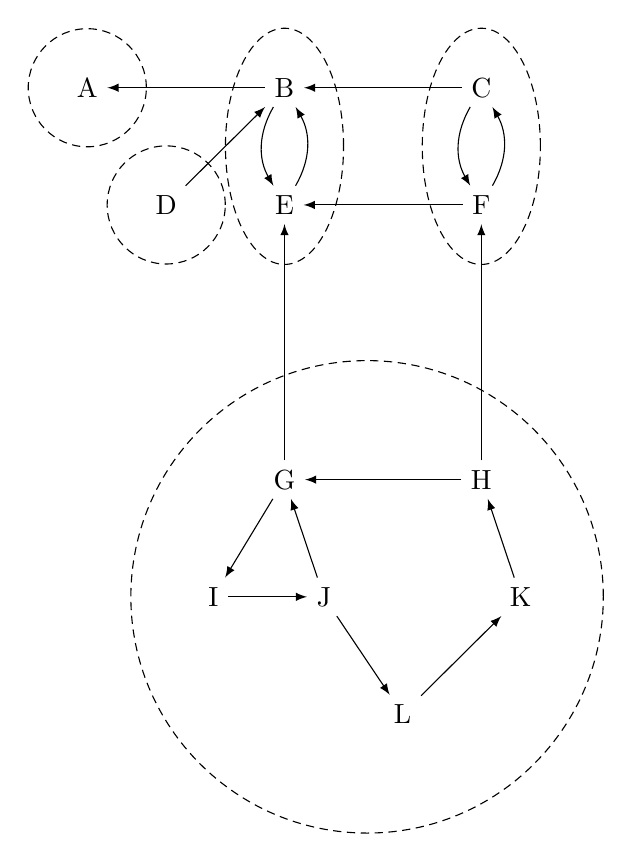
\begin{tikzpicture}
        
        %nodes
        
        \node(A) at (0,0) {A};
        \node(B)[anchor=west] at ($(A.east) + (2,0)$) {B};
        \node(C)[anchor=west] at ($(B.east) + (2,0)$) {C};
        \node(E)[anchor=north] at ($(B.south) + (0,-1)$) {E};
        \node(F) at (E-|C) {F};
        \node(D)[anchor=east] at ($(E.west) + (-1,0)$) {D};
        \node(G)[anchor=north] at ($(E.south) + (0,-3)$) {G};
        \node(H) at (G-|F) {H};
        \node(J)[anchor=north] at ($(G.south) + (0.5,-1)$) {J};
        \node(K)[anchor=north] at ($(H.south) + (0.5,-1)$) {K};
        \node(I)[anchor=east] at ($(J.west) + (-1,0)$) {I};
        \node(L)[anchor=north] at ($(J.south) + (1,-1)$) {L};
        
        %grouping circles
        
        \draw[densely dashed] (A) circle[radius=0.75cm];
        \draw[densely dashed] (D) circle[radius=0.75cm];
        \draw[densely dashed] ($(B)!0.5!(E)$) circle [x radius=0.75cm, y radius=1.5cm];
        \draw[densely dashed] ($(C)!0.5!(F)$) circle [x radius=0.75cm, y radius=1.5cm];
        \draw[densely dashed] ($(I)!0.5!(K)$) circle [radius=3cm];
        
        %arrows
        
        \draw[-latex] (B) edge (A);
        \draw[-latex] (D) edge (B);
        \draw[-latex] (C) edge (B);
        \draw[-latex] (E) edge[bend right] (B);
        \draw[-latex] (B) edge[bend right] (E);
        \draw[-latex] (F) edge[bend right] (C);
        \draw[-latex] (C) edge[bend right] (F);     
        \draw[-latex] (F) edge (E);
        \draw[-latex] (G) edge (E);
        \draw[-latex] (H) edge (F);
        \draw[-latex] (H) edge (G);
        \draw[-latex] (G) edge (I);
        \draw[-latex] (I) edge (J);
        \draw[-latex] (J) edge (G);
        \draw[-latex] (J) edge (L);
        \draw[-latex] (L) edge (K);
        \draw[-latex] (K) edge (H);
    \end{tikzpicture}9

    As we explain the issue, we also develop a 

BFS from root upwards, rank nodes based on depth. Then progress as usual. Explain code with comments.

Time complexity of my algorithm is $\mathcal{O}(n^{2}\log(n)$, with further improvements can get it to $\mathcal{O}(n\log(n))$ I think.

\end{document}